\subsection{Conceptual Class Diagram}
\newpage
\vspace*{-2.8in}
\begin{figure}[H]
\hspace*{-1.2in}
\fbox{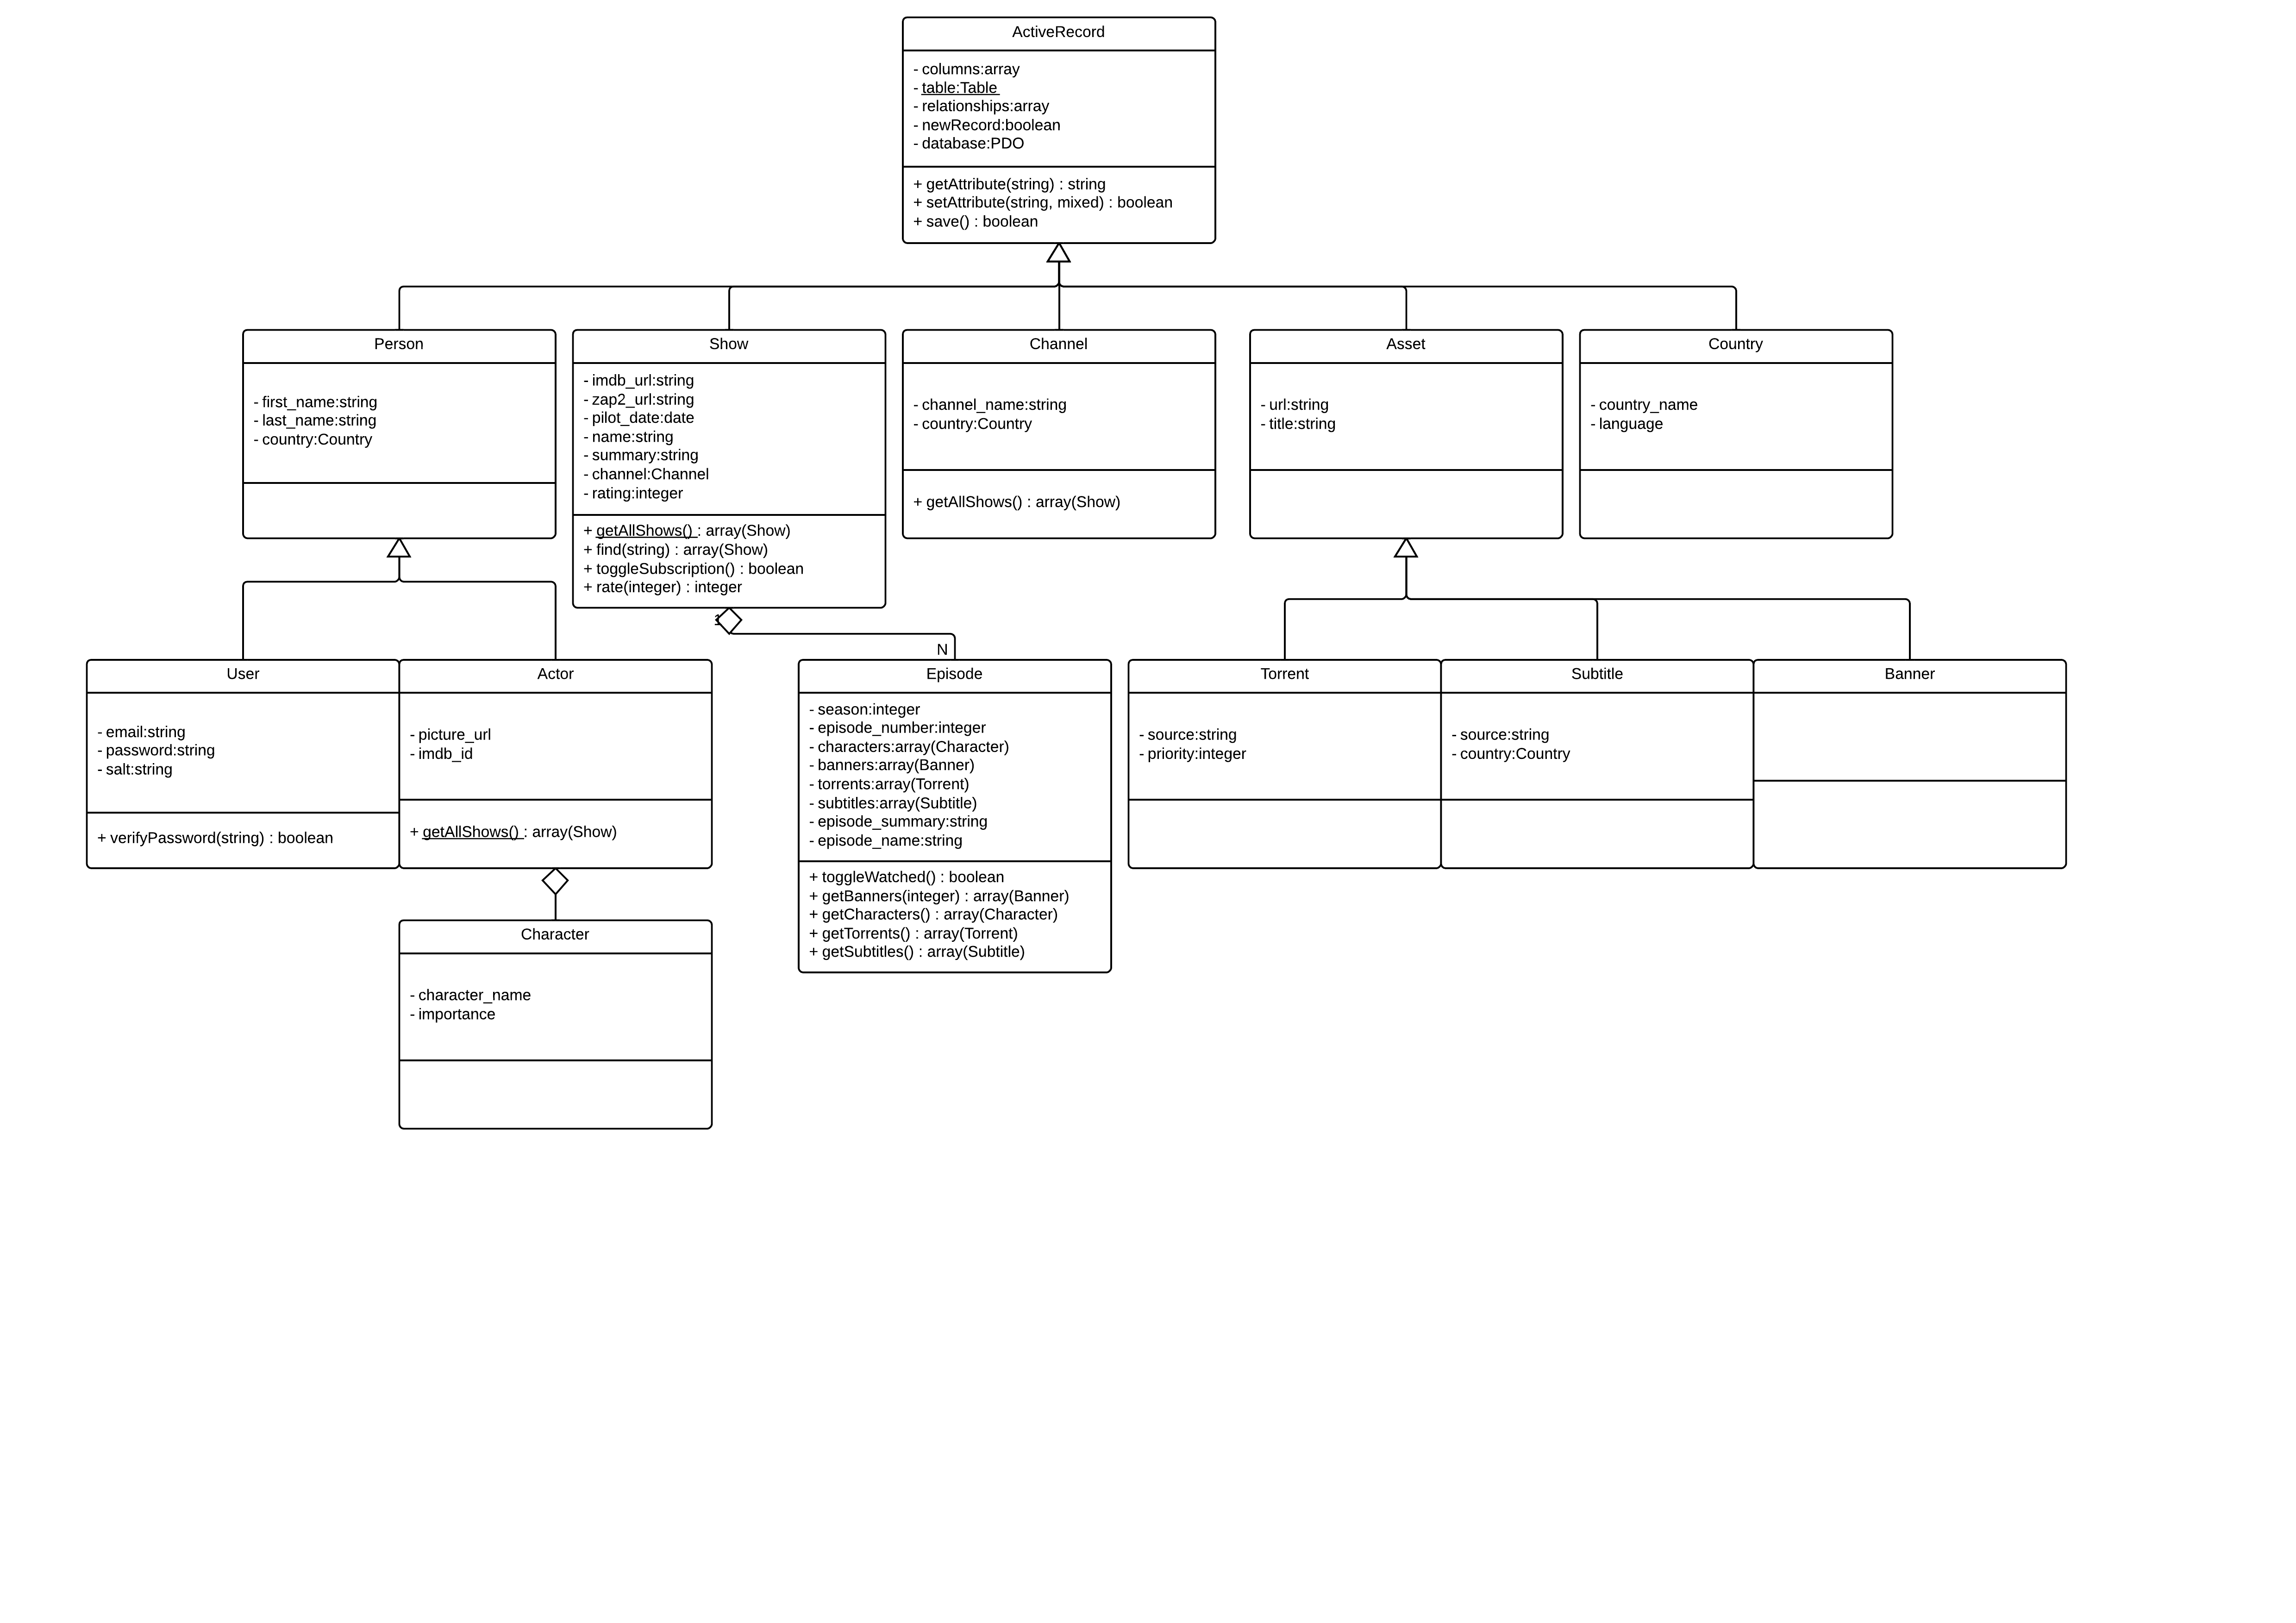
\includegraphics[scale=0.185,angle=90]{graphics/classdiagramnew}}
\caption{Conceptual Class Diagram}
\end{figure}

The conceptual class diagram illustrated above shows the most vital objects for the application and their properties and relationship to one another. Abstract classes, 3rd party library classes or classes utilized by others (such as the database handler class) are intentionally omitted here, but it serves to provide an overview of the relationships between objects within the application.

The most important objects here are \textit{User} and \textit{Show}. The main focus of the system should be on \textit{Show}, because this is the object users will interact the most with. Even without creating a user, it should be possible to browse through the list of shows and their episodes.

However, for more tailored functionality, it's of utmost importance that a \textit{User} is able to log in after being created, and that functionality is provided to allow the user to specify what shows he or she watches.

A \textit{User} may also be an administrator, or any other \textit{Role} with special permissions one may want to assign a user, and it should be possible to create and assign new \textit{Roles} at a later time.

Next, when a \textit{Show} has been selected, it's highly important that we're able to present some information about this \textit{Show}. Information that may be of interest, such as what \textit{Channel} it was originally broadcast on, information about each episode, character, or actor, needs to be retrievable from each \textit{Show} object. 

It's not unlikely that a \textit{User} would like to filter \textit{Shows} by what channel produced or first broadcast it, and as such, it should be possible to retrieve a list of \textit{Shows} from a \textit{Channel} object.

If a \textit{User} has found a \textit{Show} he or she may want to watch, it's very likely that he or she will begin to look for a way to download or stream it. It's therefore desired that lists of \textit{Torrents} and \textit{Subtitles} can be presented for any given \textit{Episode} of any given \textit{Show}.

Furthermore, when a \textit{User} views an \textit{Episode}, he or she may be interested in knowing what \textit{Characters} exist and maybe more importantly, what \textit{Actors} play in this \textit{Episode}, and therefore it's important that a list of \textit{Characters} (sorted by their \textit{importance}) and what \textit{Actors} plays them can be retrieved and presented to the \textit{User}.
\newpage